\section{Application fil rouge : le réseau local domestique}\label{sec:introduction:digitalhome}
Cette thèse a été développé dans un milieu industriel chez \textit{Orange France Telecom}. Ainsi, le travail a été motivé par une application pratique posant actuellement de nombreux problèmes en terme de compréhension : le réseau local domestique (ou \textit{Digital Home}).

\begin{figure}[ht]
\centering
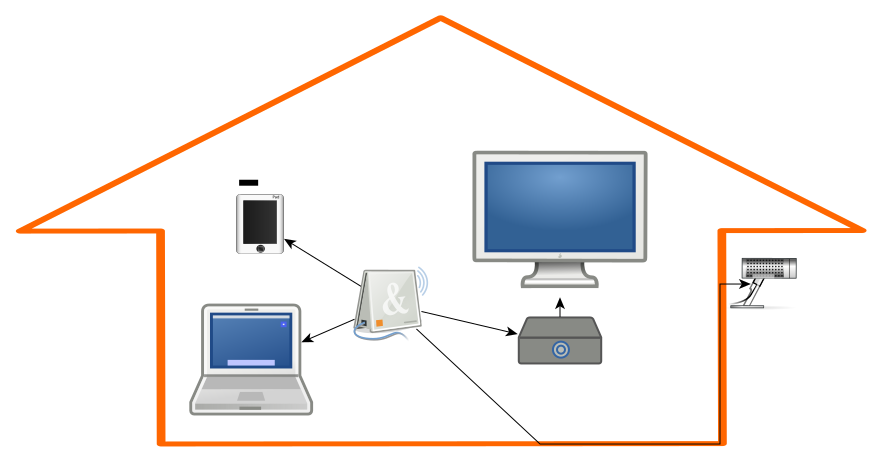
\includegraphics[width=0.7\textwidth]{intro-digitalhome}
\caption{Exemple de réseau local domestique}
\end{figure}

Le réseau local domestique est le réseau formé par l'ensemble des appareils d'un utilisateur dans sa maison. Ce réseau est déjà capable de fournir des services tels que le partage de contenus entre un disque dur en réseau (ou \textit{NAS}) sur la télévision ou sur les ordinateurs. L'étape suivante du développement de cette approche est l'introduction de capteurs et d'actuateurs pour effectuer de la domotique.

Néanmoins, il n'est pas nécessaire de créer un tel cas d'usage pour soulever des problèmes. En effet, en l'état actuel, les opérateurs qui fournissent des équipements et des services sont bien souvent impuissants pour dépanner les utilisateurs. Une raison claire de ce problème est notamment le manque d'informations. Le service après-vente est en effet incapable de connaître la topologie du réseau (utilisation de \textit{wifi} ou courant porteur), la configuration de certains équipements (notamment ceux qu'il ne maîtrise pas) et évidemment encore moins l'état de santé des équipements, des liens réseaux ou des services.

Ce cadre applicatif est utilisé tout au long de ce manuscrit. En effet, cette application possède toutes les caractéristiques que nous avons présenté dans nos problématiques.
\begin{itemize}
	\item La caractéristique principale de ce réseau est qu'il est composé de dispositifs hétérogènes.
	\item Les paramètres de configurations et d'autres données accessibles via des services spécifiques sont des données archivés. Nous sommes aussi capable de récupérer des données de métriques pour mesurer la santé du réseau. Les deux sont nécessaires pour établir une observation unifié.
	\item Le système est déjà défini et fournit ses propres données. Chaque équipement peut fournir des données diverses qu'il nous faut intégrer.
	\item L'écosystème a ses propres caractéristiques et il faut nous adapter à son fonctionnement. Notamment, certains équipements sont limités en terme de capacités de traitement.
\end{itemize}